\clearpage
\section{Obtained Cross-section Upper-limit}
$\mathrm{CL_s}$ value is calculated as the function of the signal strength $\mu (\in [0,5])$ in the hypothetical test. Therefore, the upper limit on $\mu$ can be determined as:
\begin{align}
\mu_{95\mathrm{CL}} := \mu(\mathrm{CL_s}=0.05).
\end{align}
This can be straightforwardly interpreted into the upper limit on the excluded cross-section ($\sigma_{95\mathrm{CL}}$), and it is a completely model-independent presentation of the result once the decay chain and the masses of gluino and EW-gauginos are specified.
Figure \ref{fig::Result::xsecUL::QQC1QQC1}-\ref{fig::Result::xsecUL::TTN1TTN1} present the results for the reference models \textbf{QQC1QQC1}, \textbf{QQC1BTC1} and \textbf{TTN1TTN1}. \\
%, and the full result are in the Appendix \ref{sec::Result::xsecUL::nonBenchMark}.

\clearpage
%% -- xsec UL ----------------------
\begin{figure}[h]
  \centering
%    \subfigure[]{\includegraphics[width=0.48\textwidth]{figures/Result/xsecUL/onestepCC_x12.pdf}}
%    \subfigure[]{\includegraphics[width=0.48\textwidth]{figures/Result/xsecUL/onestepCC_varx.pdf}}
    \subfigure[]{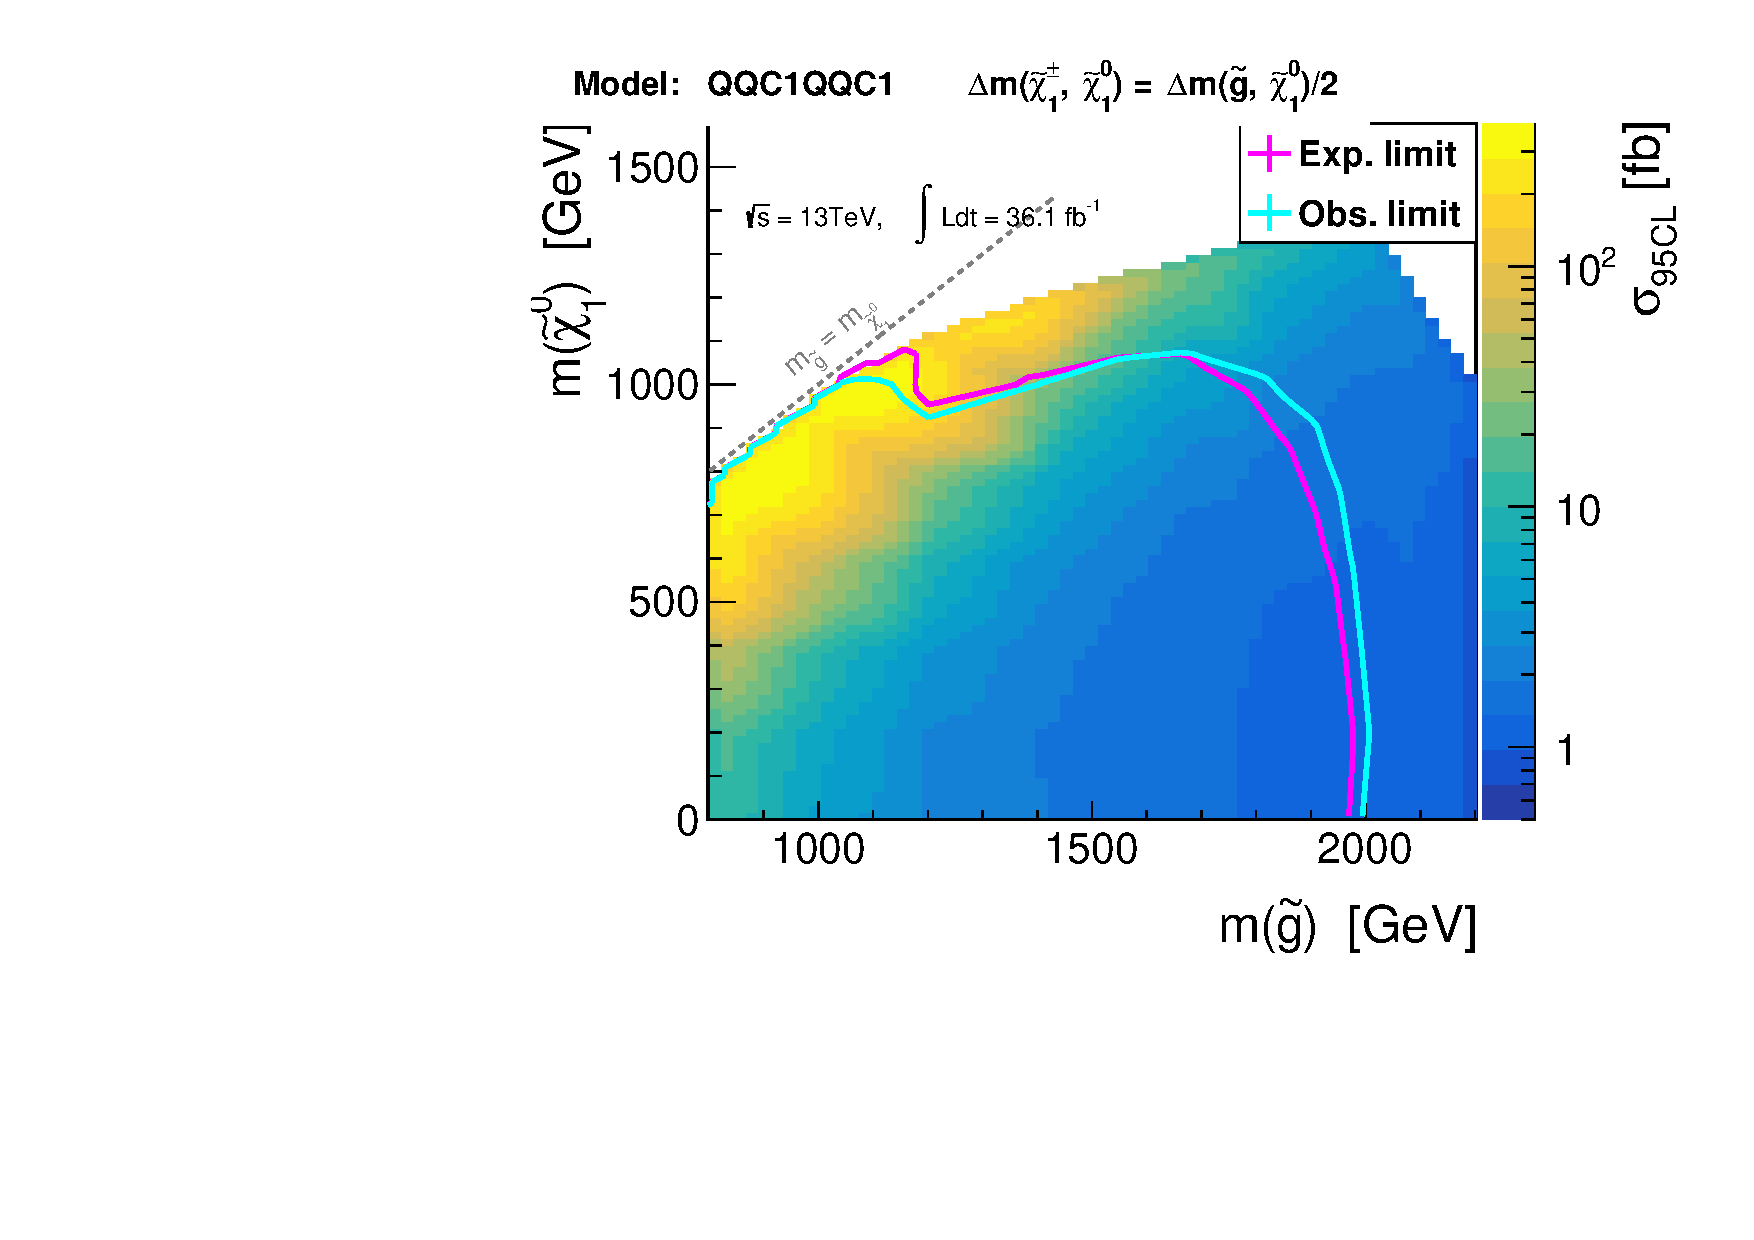
\includegraphics[width=0.48\textwidth]{figures/Result/xsecUL/symQQC1_x12.pdf}}
    \subfigure[]{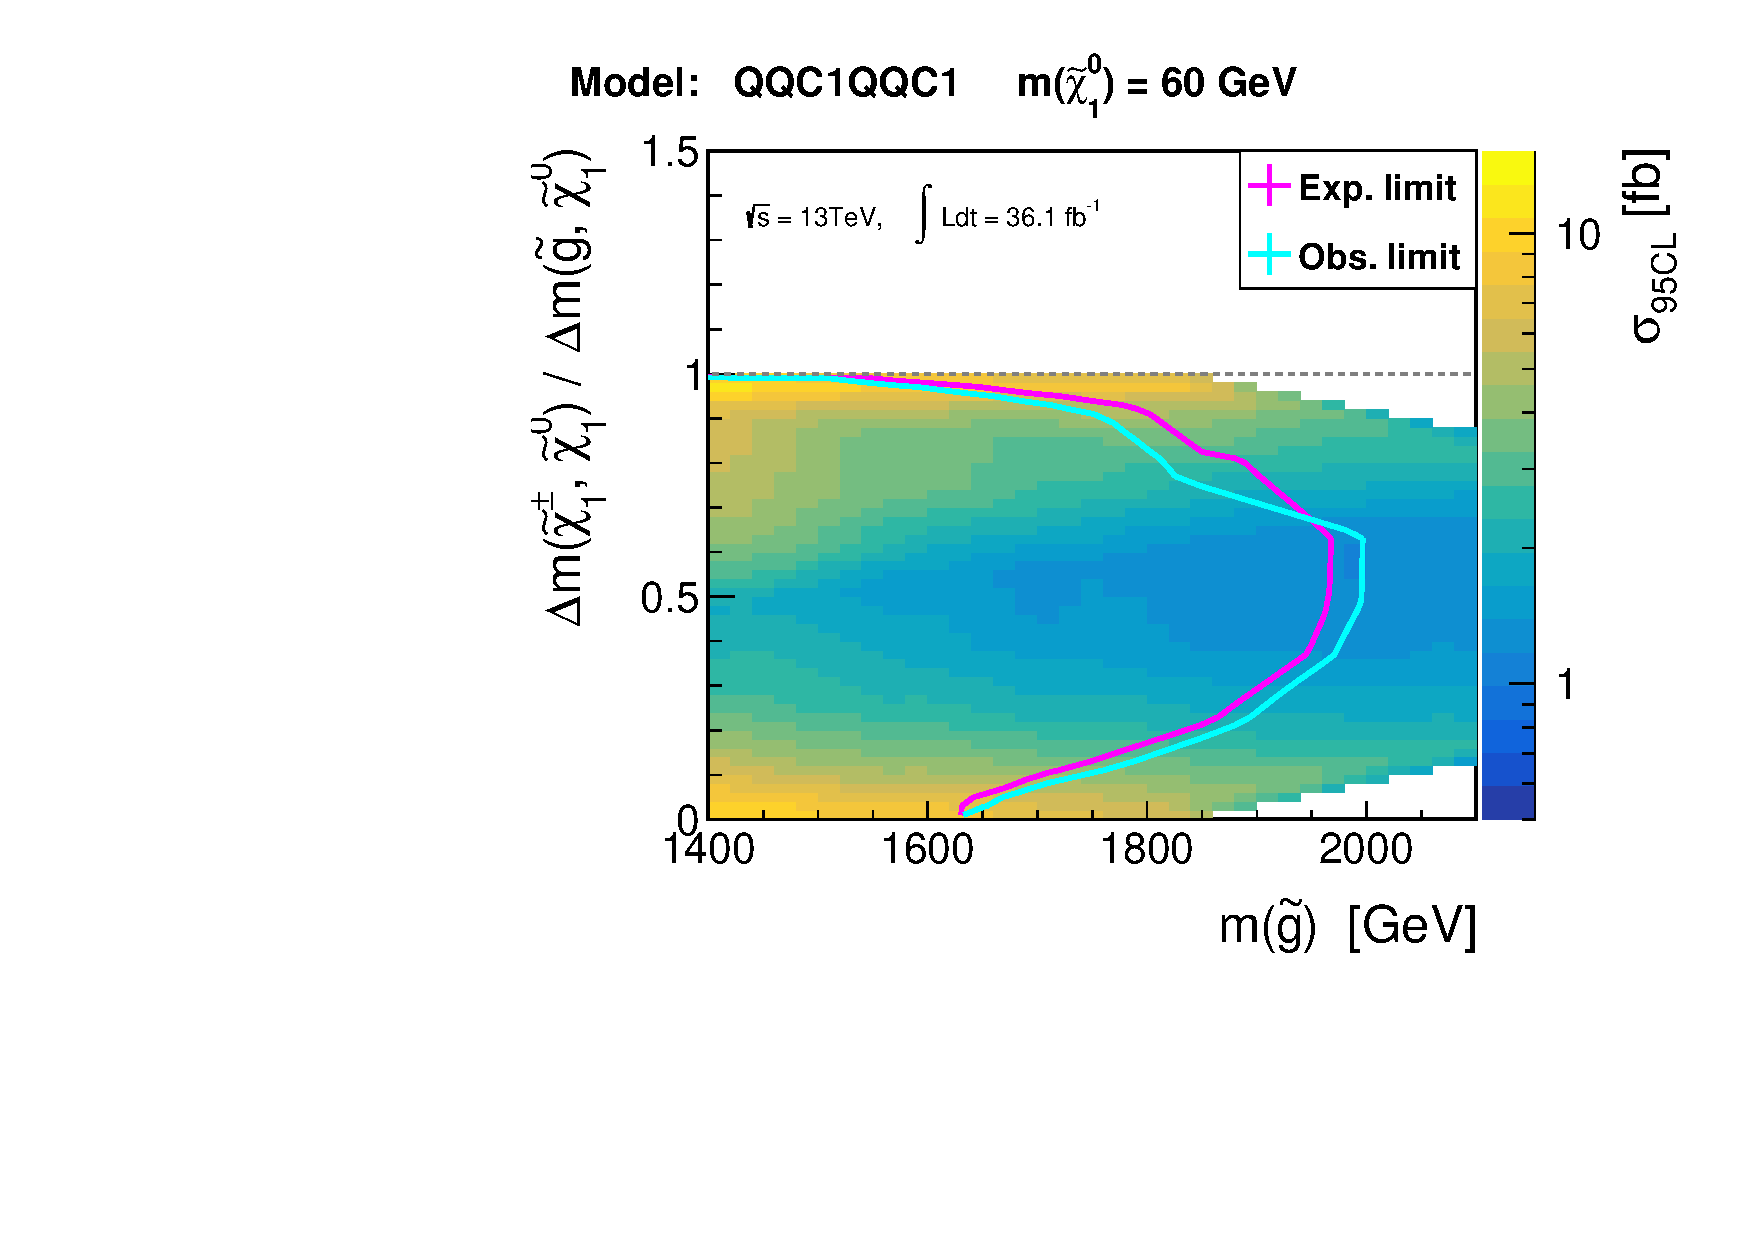
\includegraphics[width=0.48\textwidth]{figures/Result/xsecUL/symQQC1_varx.pdf}}
    \subfigure[]{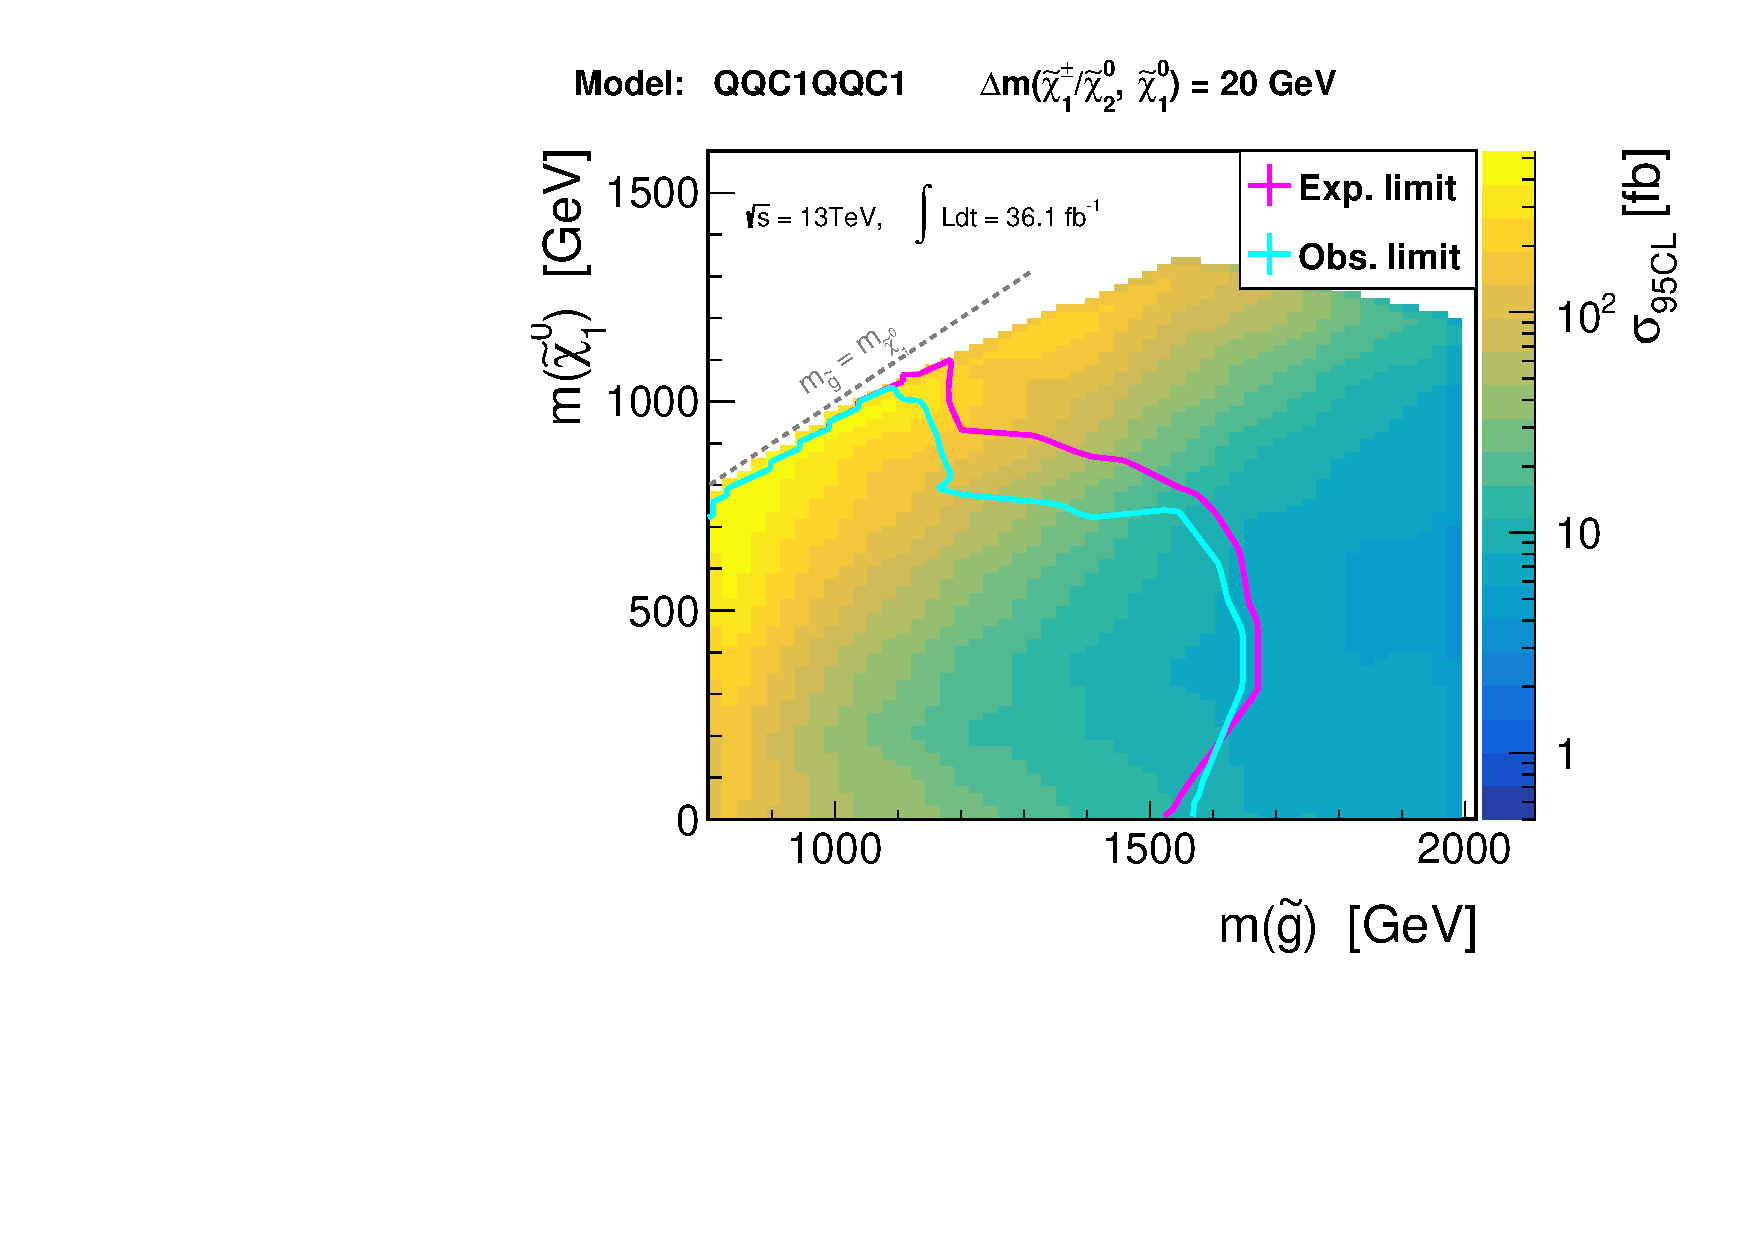
\includegraphics[width=0.48\textwidth]{figures/Result/xsecUL/symQQC1_dM20.pdf}}
    \subfigure[]{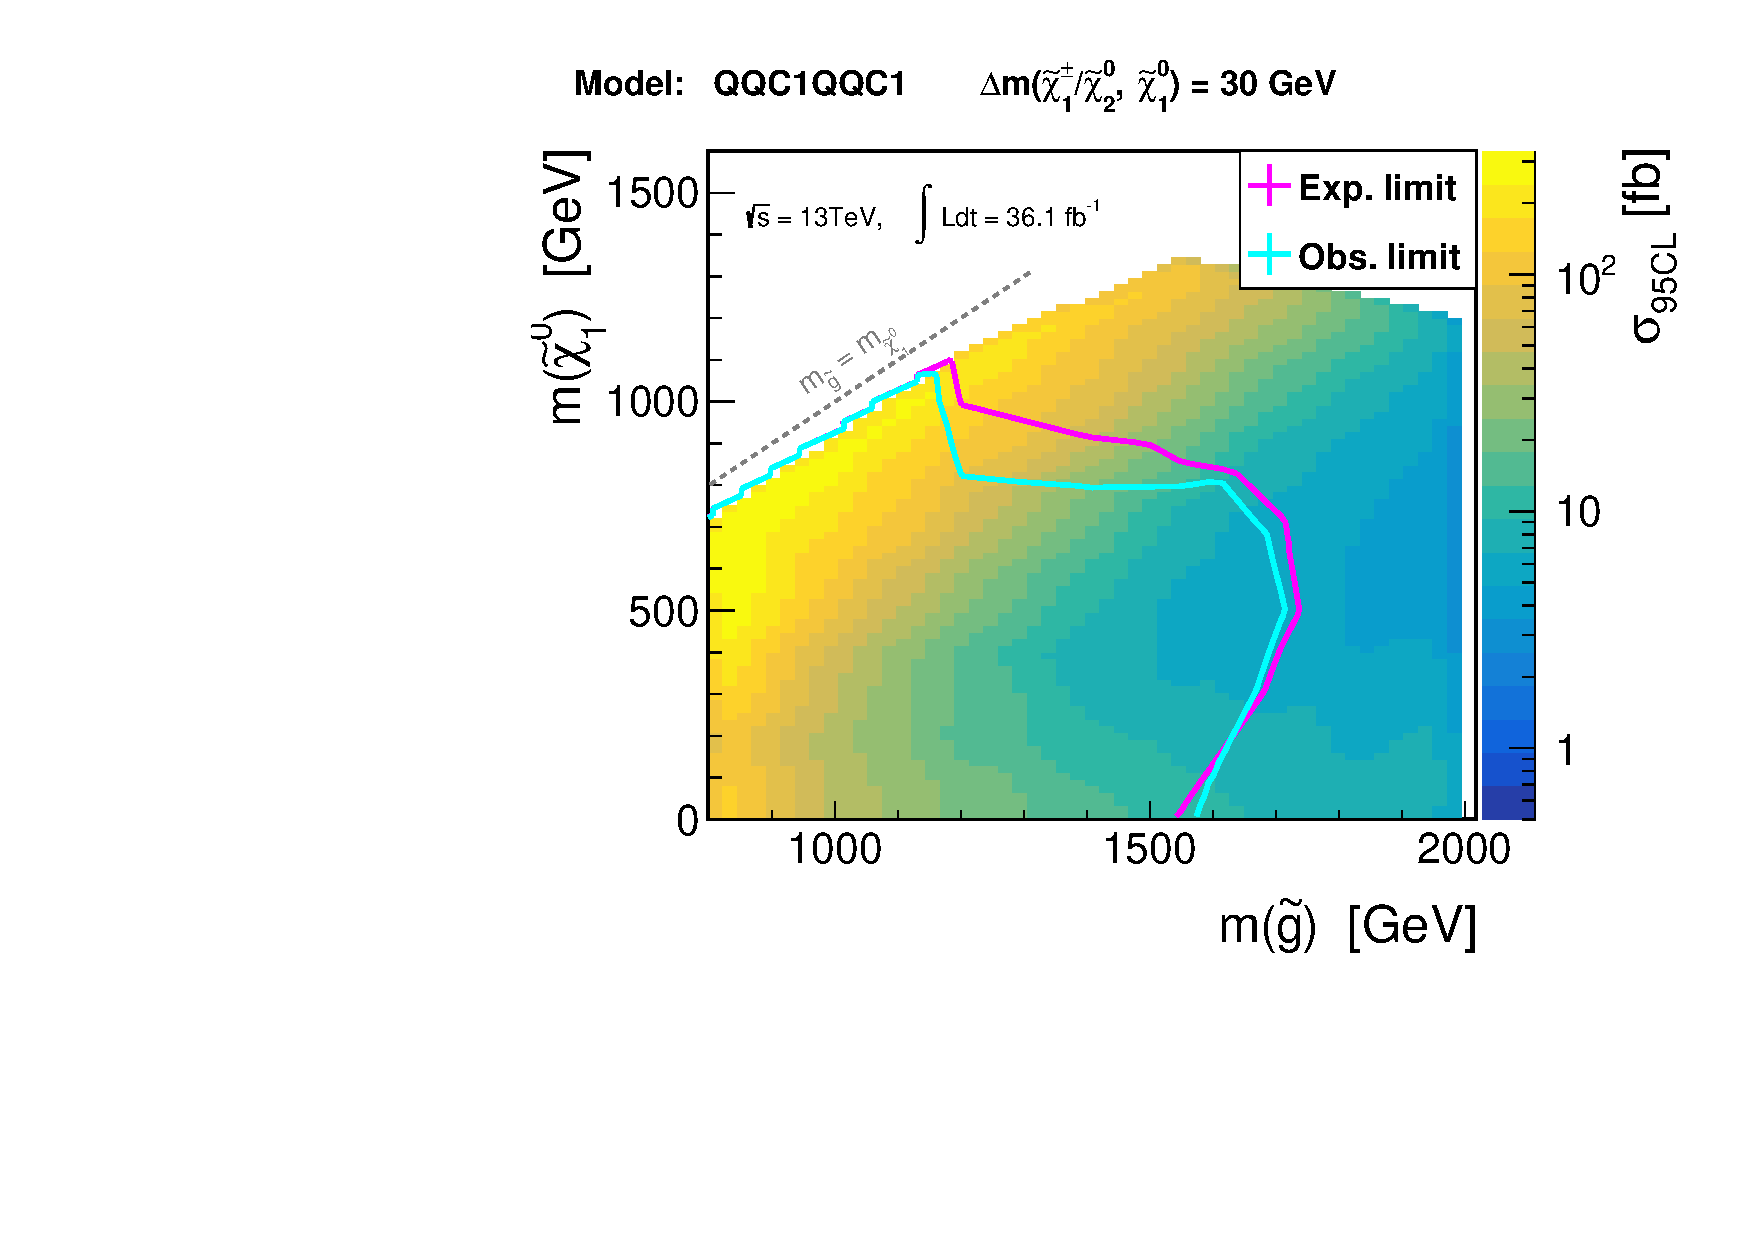
\includegraphics[width=0.48\textwidth]{figures/Result/xsecUL/symQQC1_dM30.pdf}}
    \caption{
    Upper limit of excluded cross-section (95$\%$CL) as the function of the SUSY masses, for benchmark model \textbf{QQC1QQC1}, presented in the grids (a) $x=1/2$ (b) $\mLSP=60\gev$ (c) $\dmc=20\gev$ (d) $\dmc=30\gev$.
    \label{fig::Result::xsecUL::QQC1QQC1} }
\end{figure}


%figures/Result/xsecUL/symQQC1_dM20.pdf

%% --
\begin{figure}[h]
  \centering
    \subfigure[]{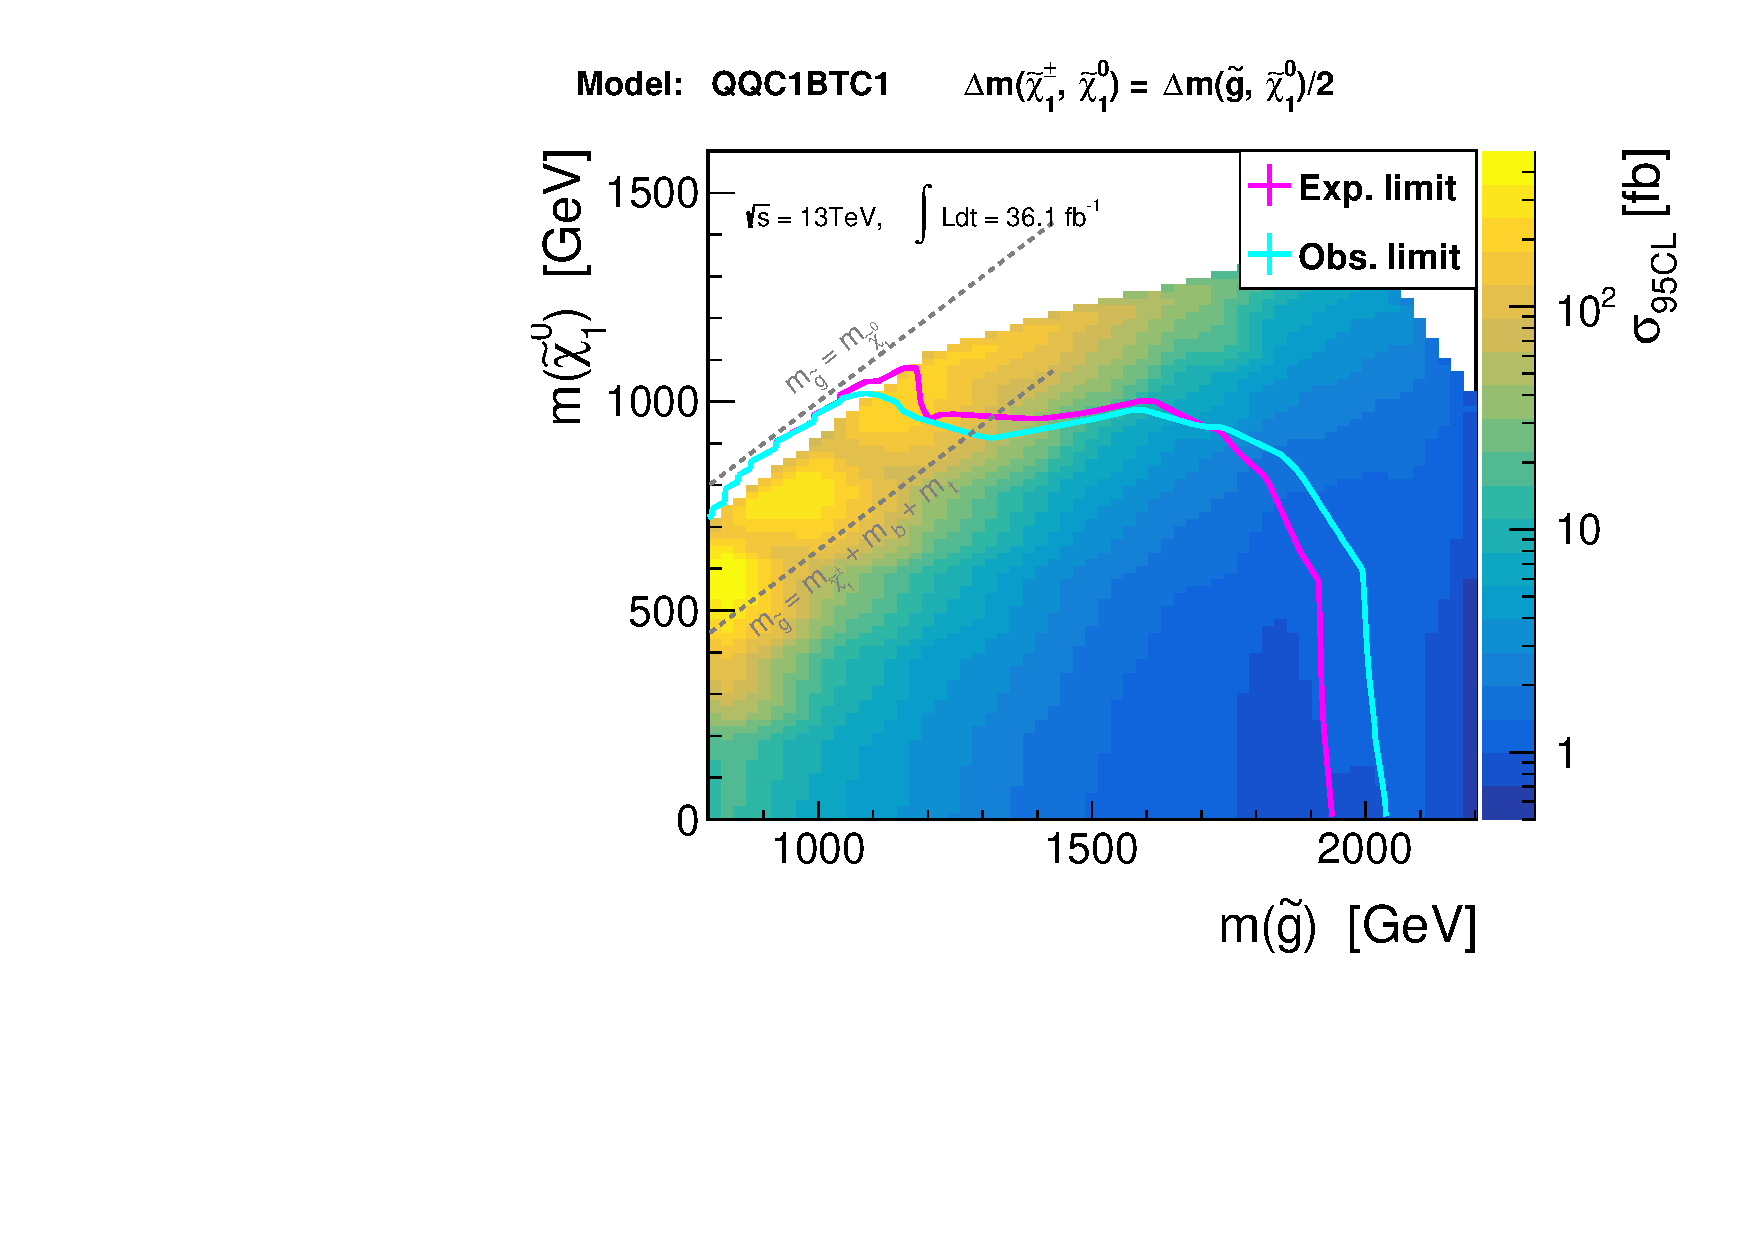
\includegraphics[width=0.48\textwidth]{figures/Result/xsecUL/QQC1BTC1_x12.pdf}}
    \subfigure[]{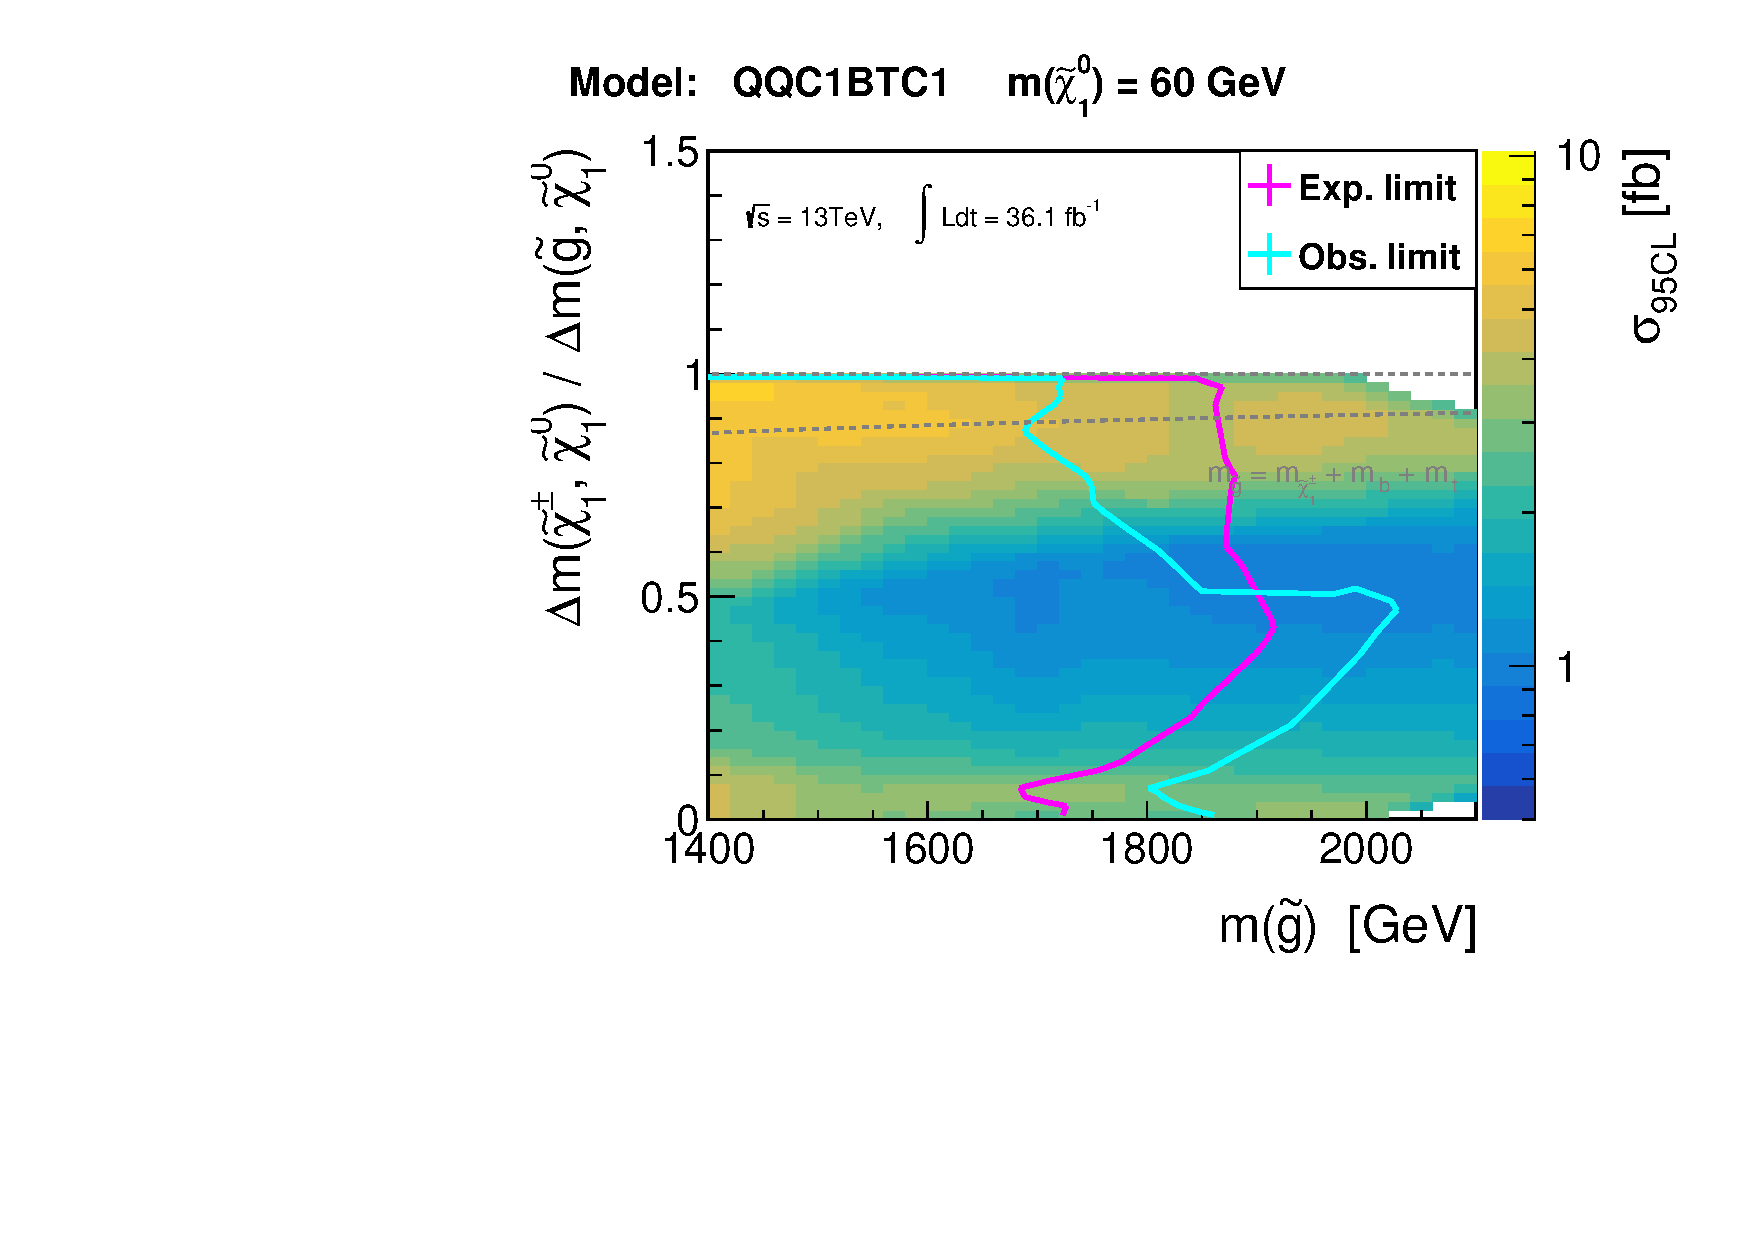
\includegraphics[width=0.48\textwidth]{figures/Result/xsecUL/QQC1BTC1_varx.pdf}}
    \subfigure[]{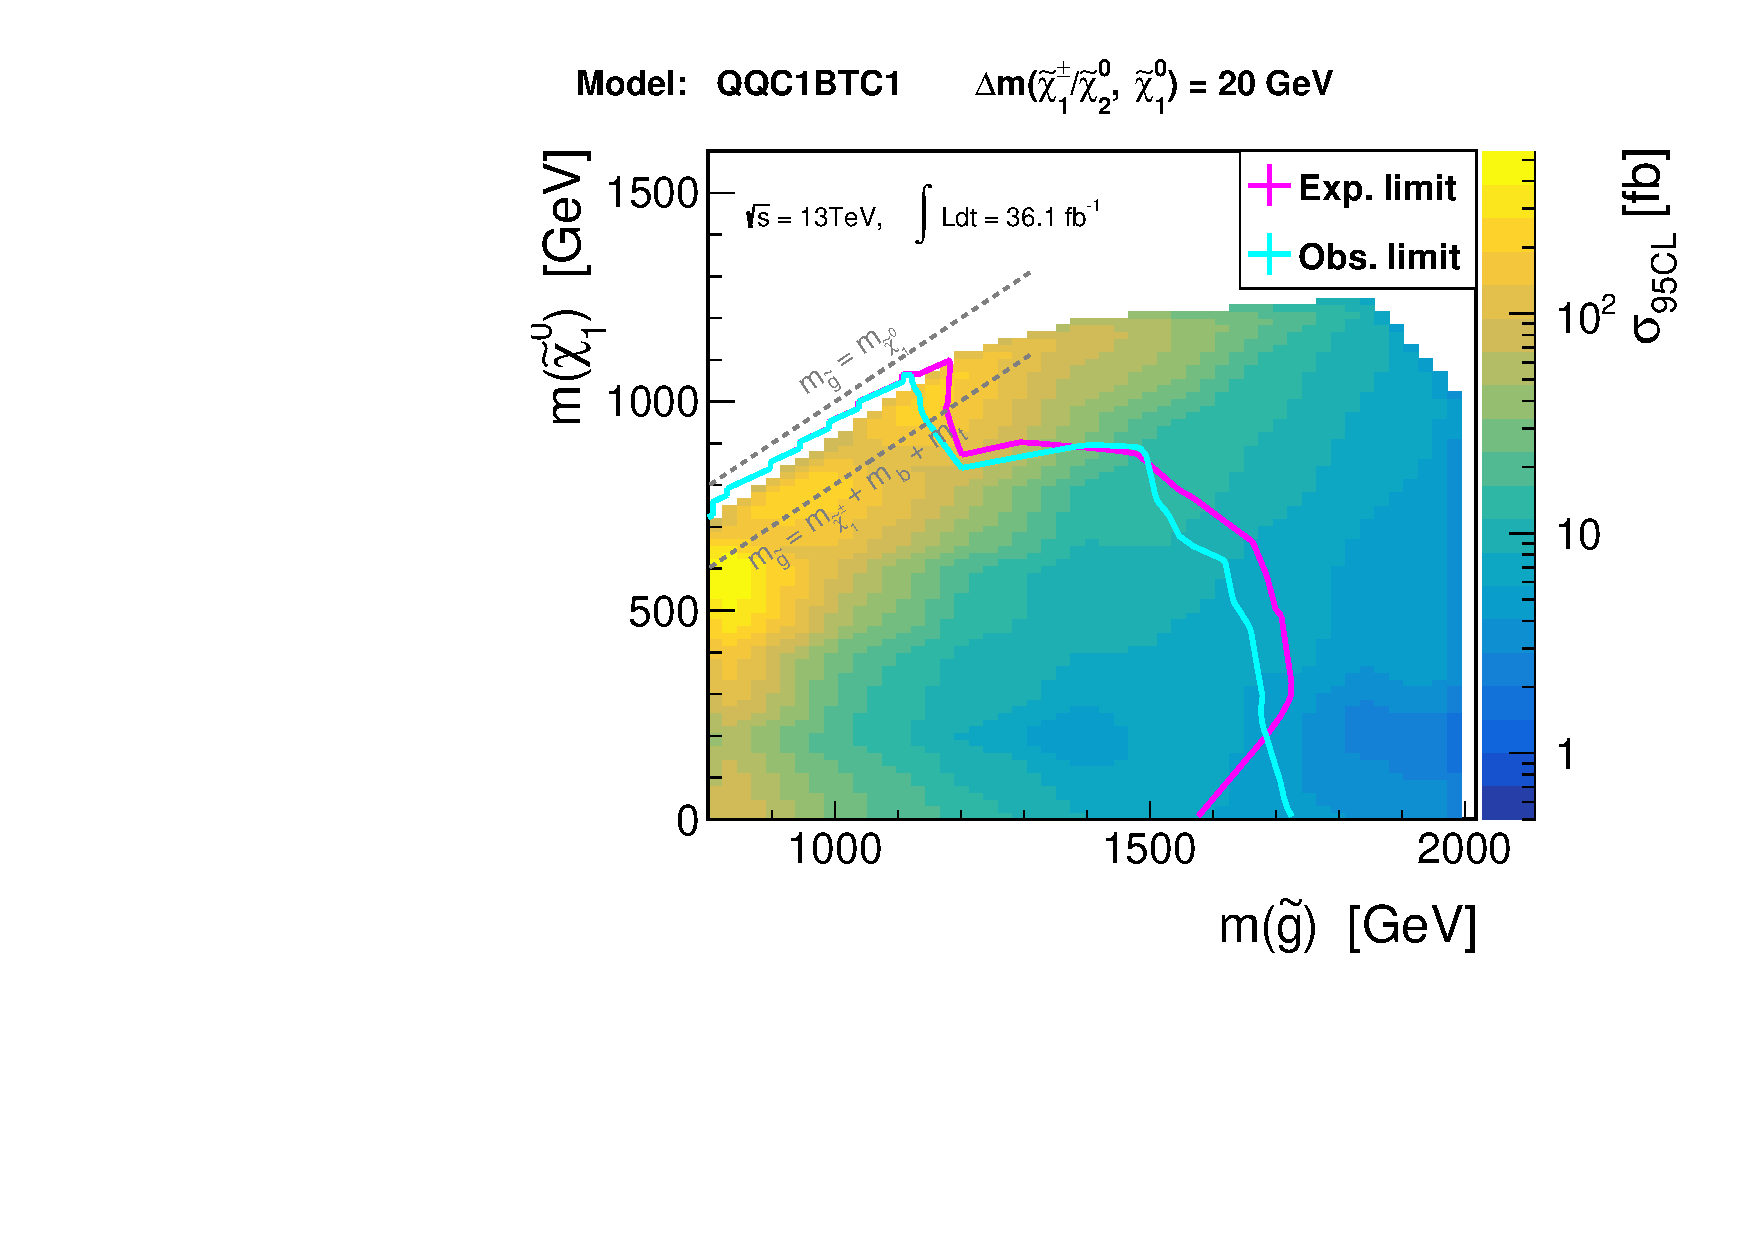
\includegraphics[width=0.48\textwidth]{figures/Result/xsecUL/QQC1BTC1_dM20.pdf}}
    \subfigure[]{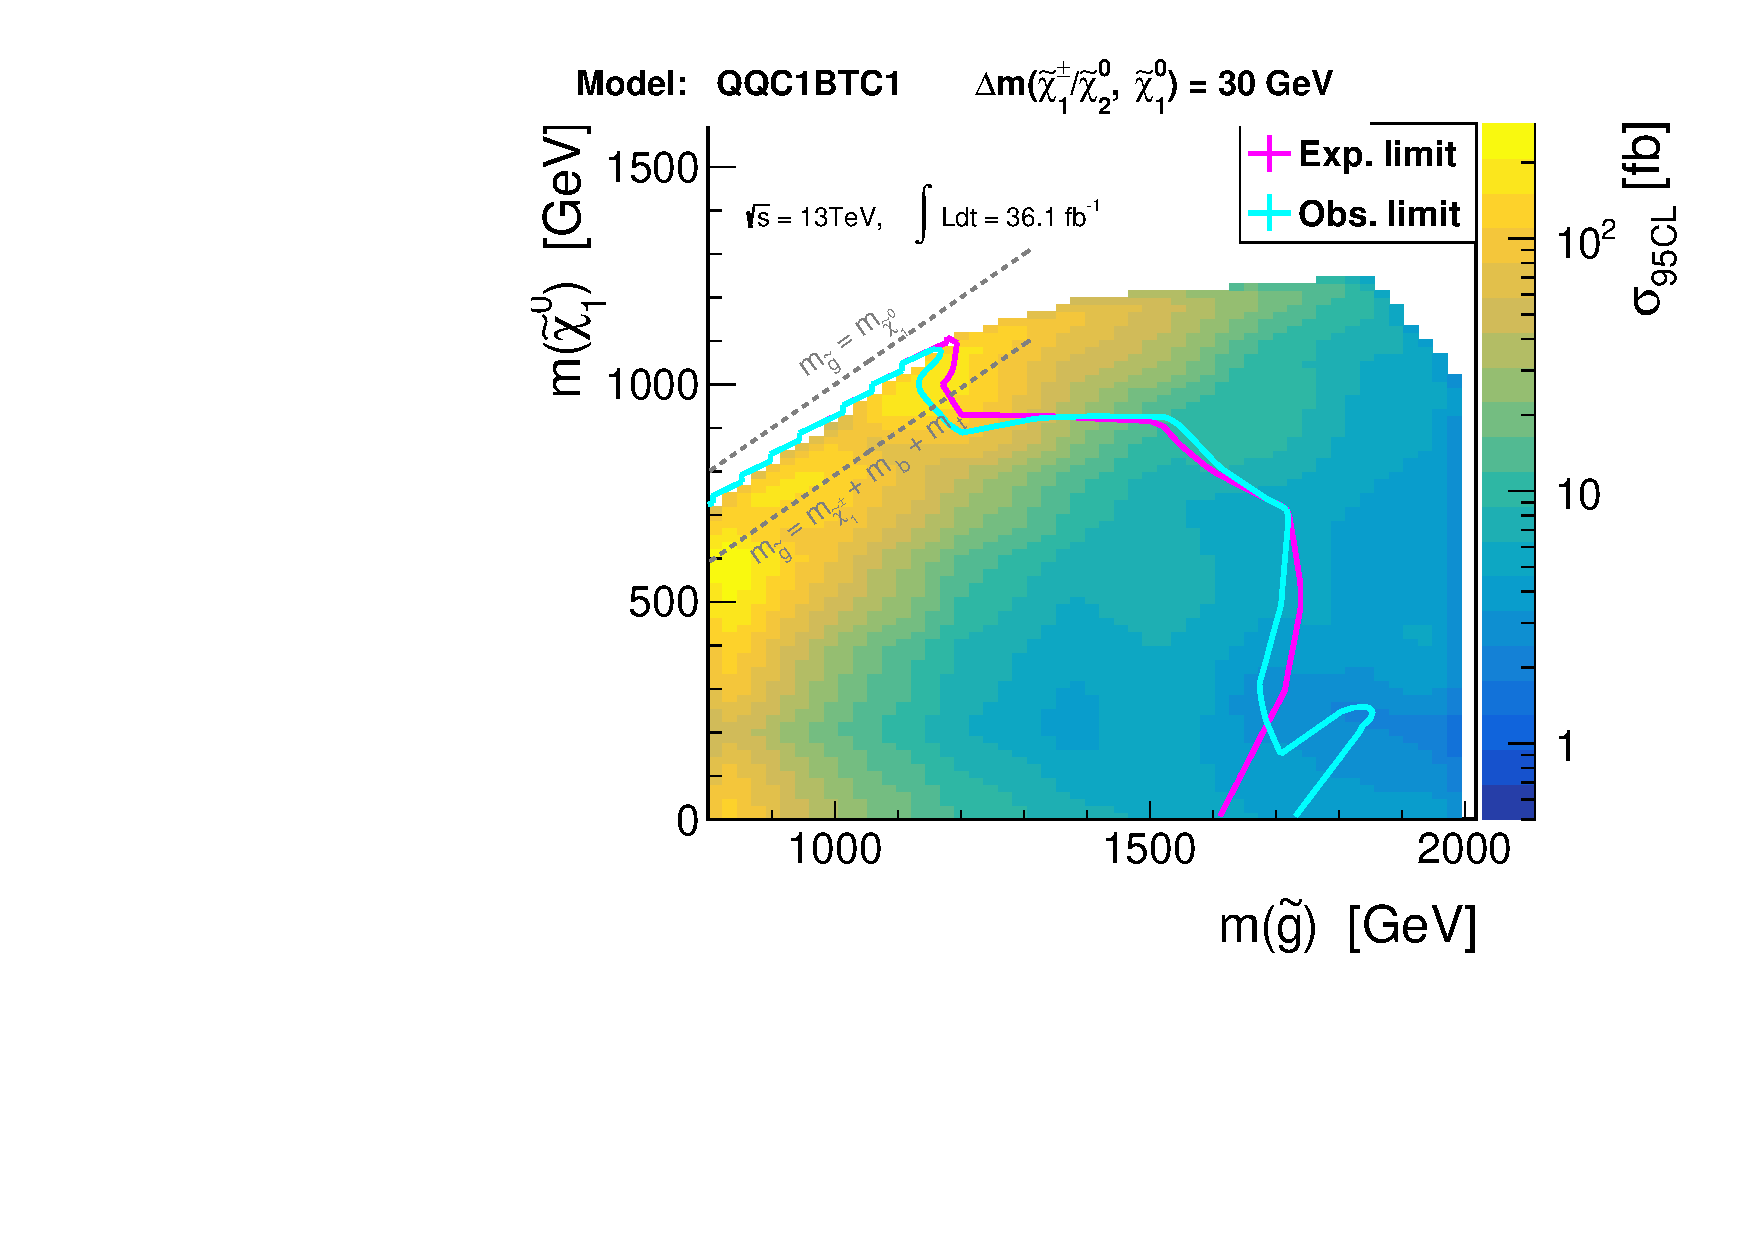
\includegraphics[width=0.48\textwidth]{figures/Result/xsecUL/QQC1BTC1_dM30.pdf}}
    \caption{
    Upper limit of excluded cross-section (95$\%$CL) as the function of the SUSY masses, for benchmark model \textbf{QQC1BTC1}, presented in the grids (a) $x=1/2$ (b) $\mLSP=60\gev$ (c) $\dmc=20\gev$ (d) $\dmc=30\gev$.
    \label{fig::Result::xsecUL::QQC1BTC1} }
\end{figure}

%% --
\begin{figure}
  \begin{center}
    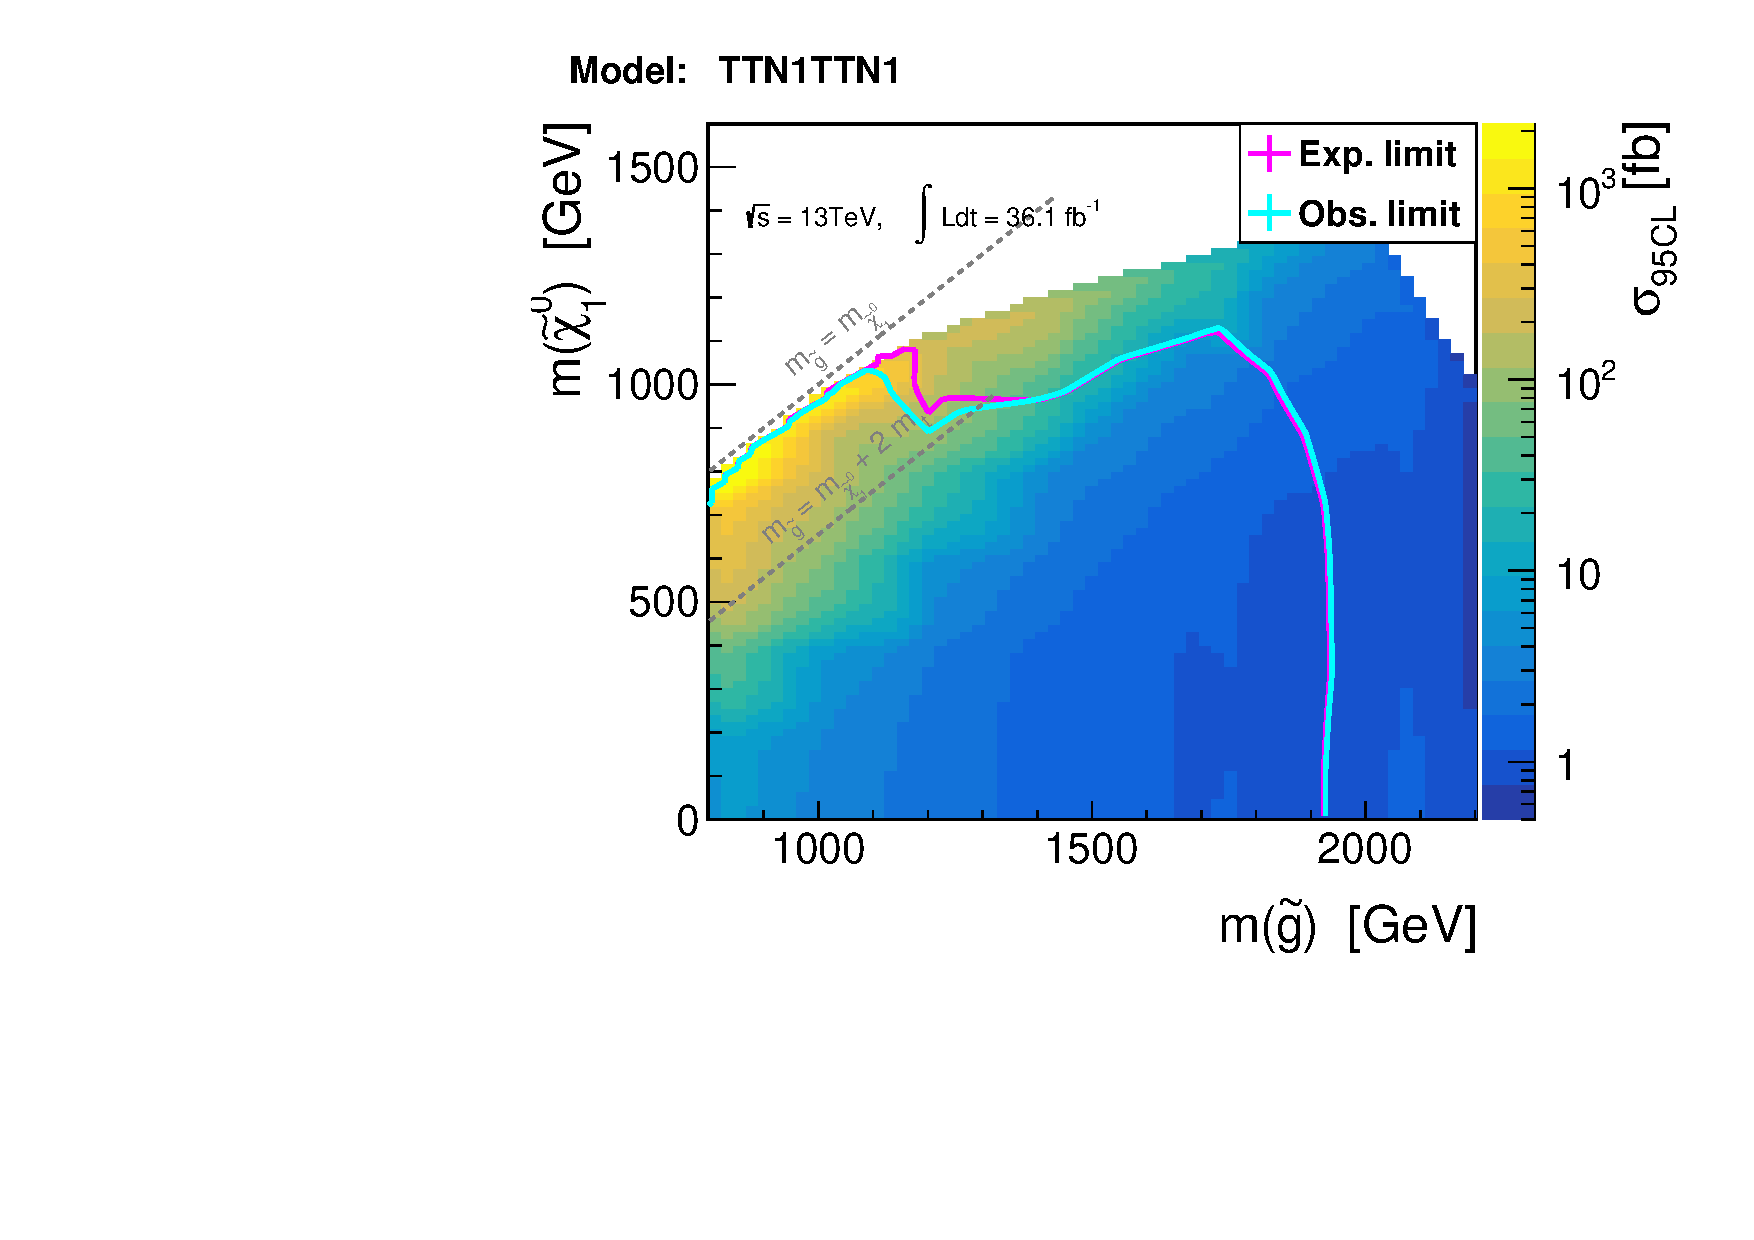
\includegraphics[width=160mm]{figures/Result/xsecUL/symTTN1_x12.pdf}
    \captionof{figure}{
    Upper limit of excluded cross-section (95$\%$CL) as the function of the SUSY masses, for benchmark model
 \textbf{TTN1TTN1}.
    \label{fig::Result::xsecUL::TTN1TTN1} }       
  \end{center}
\end{figure}
%-------------------------------                                                                                                   

